\documentclass[11pt]{article}
\usepackage{tikz}
\usepackage{endiagram}
\usepackage{chemmacros}
\usetikzlibrary{automata,positioning,arrows}
\usepackage{siunitx}
\begin{document}


\begin{endiagram}[
tikz = {yscale=1.2}, scale = 1.0,
energy-step=50,
%energy-zero=-200,
energy-unit=\kilo\joule\per\mole,
%AddAxisLabel/font = \footnotesize,
y-label = above, y-label-text = $\Delta H$,
x-label= below, x-label-text = Progresso da Reação]
%\ENcurve{2,3,1}
\ENcurve{0,0,0,3,-4.5,-4.5,-4.5}
\AddAxisLabel*{-5;-4;-3;-2;-1;0;1;2;3;4}
\draw(1.7,.8)node{\ch{CO_{\gas} + NO2_{\gas}}};
\draw(10.5,-3.9)node{\ch{CO2_{\gas} + NO_{\gas}}};
%\draw[dashed,help lines] (N1-2) -- (N1-2 -| origin-l) node[left,blue] {} ;
\AddAxisLabel{(N1-2)}
\end{endiagram}


\newpage

\begin{reactions*}
CaCO3_{\sld} -> CO2_{\gas} + CaO_{\sld} & $\qquad \enthalpy{178}$ \\
CaO_{\sld}   
\end{reactions*}

Observe o diagrama a seguir
\begin{center}
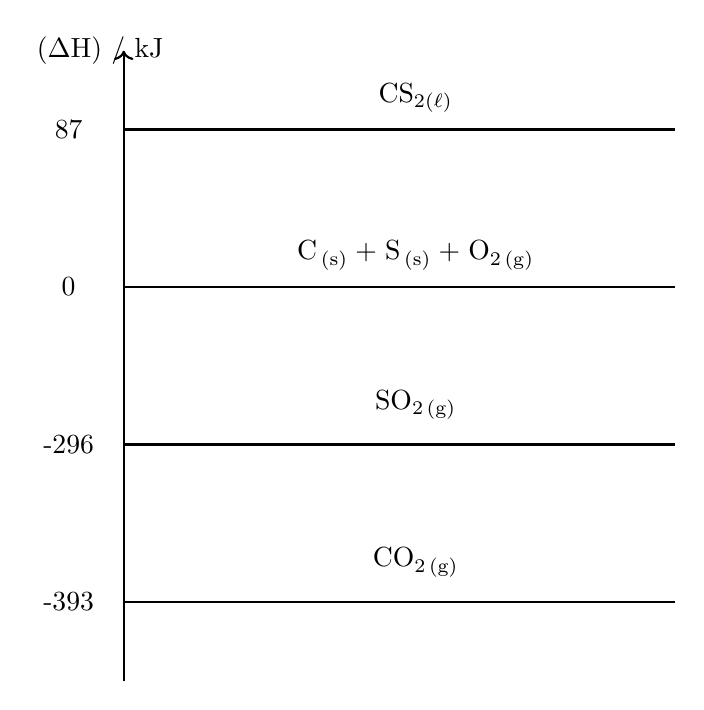
\begin{tikzpicture}
\draw[thick,->](0,0) -- (0,8);
\draw(-.3,7.7) node[sloped,anchor=center, rotate=0, above]{($\Delta$H) / kJ};
%Line 1
\draw[thick,-](0,7) -- (7,7);
\draw(-0.7,7) node{87};
\draw(3.7,7.4) node{\ch{CS2_{($\ell$)}}};
%% Line 2
\draw[thick,-](0,5) -- (7,5);
\draw(-0.7,5) node{0};
\draw(3.7,5.4) node{\ch{C_{\sld} + S_{\sld} + O2_{\gas}}};
%%% Line 3
\draw[thick,-](0,3) -- (7,3);
\draw(-0.7,3) node{-296};
\draw(3.7,3.5) node{\ch{SO2_{\gas}}};
%%%%% Line 4
\draw[thick,-](0,1) -- (7,1);
\draw(-0.7,1) node{-393};
\draw(3.7,1.5) node{\ch{CO2_{\gas}}};
\end{tikzpicture}
\end{center}
Qual o valor da entalpia da reação para a reação a seguir.
\begin{reaction*}
CS2_{\lqd} + 3 O2_{\gas} -> CO2_{\gas} + 2 SO2_{\gas}
\end{reaction*}

\newpage


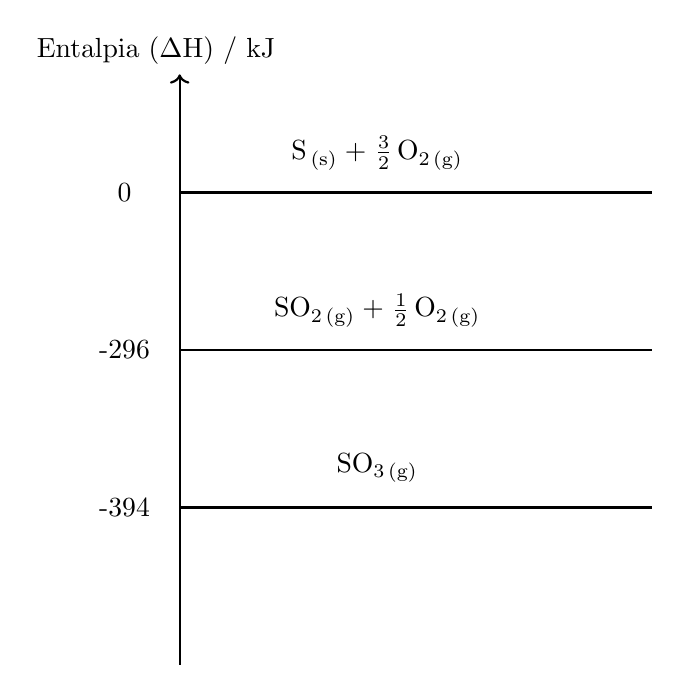
\begin{tikzpicture}[scale=1]
%\draw[step=1cm,black,very thin] (0,0) grid (10,10);
\draw[thick,->](0,0) -- (0,7.5);
\draw(-.3,7.5) node[sloped,anchor=center, rotate=0, above]{Entalpia ($\Delta$H) / kJ};
%% Line 1
\draw[thick,-](0,2) -- (6,2);
\draw(-0.7,2) node{-394};
\draw(2.5,2.5) node{\ch{SO3_{\gas}}};
%%% Line 2
\draw[thick,-](0,4) -- (6,4);
\draw(-0.7,4) node{-296};
\draw(2.5,4.5) node{\ch{SO2_{\gas} + 1/2 O2_{\gas}}};
%%% Line 3
\draw[thick,-](0,6) -- (6,6);
\draw(-0.7,6) node{0};
\draw(2.5,6.5) node{\ch{S_{\sld} + 3/2 O2_{\gas}}};
\end{tikzpicture}
\newpage






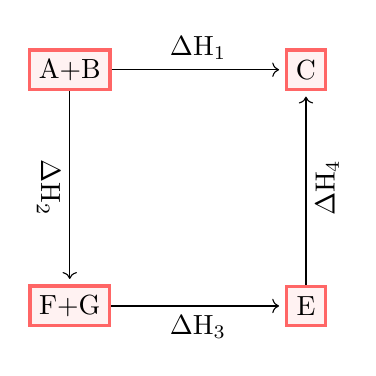
\begin{tikzpicture}[
squarednode/.style={rectangle, draw=red!60, fill=red!5, very thick, minimum size=5mm}, shorten >=2pt,node distance=3cm,on grid,
]
\node[squarednode] (1) {A+B};
\node[squarednode] (2) [right=of 1] {C};
\node[squarednode] (3) [below=of 1] {F+G};
\node[squarednode] (4) [right= of 3] {E};
%%% 
%% Lines
\draw[->] (1.east) -- node[above]{$\Delta$H$_1$}(2.west);
\draw[->] (1.south) -- node[sloped, anchor=center, below]{$\Delta$H$_2$}(3.north);
\draw[->] (3.east) -- node[below]{$\Delta$H$_3$}(4.west);
\draw[->] (4.north) -- node[sloped, anchor=center, below]{$\Delta$H$_4$}(2.south);
\end{tikzpicture}



\begin{endiagram}[
x-label=right,
y-label= above, y-label-text = Energia,
x-label= below, x-label-text = Progresso da Reação]
\ENcurve{4,4,4,-1,-1,-1}
\end{endiagram}


$\Delta$H$_1$ + $\Delta$H$_2$ + $\Delta$H$_4$


\end{document}

